% ----------------------------------------------------------------------
%  Pracovní úkoly
% ----------------------------------------------------------------------
\section{Pracovní úkoly}

\textbf{Pracovní úkol 1}

Sestavte malý laboratorní palivový článek pomocí komerčních katalytických GDE (0,3 mgPt cm-2), membrány Nafion NR212 a grafitových bipolárních desek.

\begin{enumerate}
\item Odřízněte dva kusy GDE 2×2 $cm^2$ pomocí nože a pravítka.
\item Odřízněte jeden kus membrány NR-212 7,5×4 $cm^2$.
\item Vytvořte otvory v membráně pro upínací tyče a průchod plynu.
\item Odstraňte z membrány dvě ochranné fólie.
\item Vezměte katodovou bipolární desku.
\item Položte jeden kus GDE na bipolární desku (stranou uhlíkového papíru k průtokovému poli).
\item Zakryjte membránou a zajistěte upevňovacími tyčemi.
\item Umístěte druhý kus GDE (stranou uhlíkového papíru od membrány).
\item Celý systém zakryjte anodovou bipolární deskou.

\end{enumerate}

\textbf{Pracovní úkol 2}

Nastavte experimentální prostředí pro sestavený palivový článek, aktivujte palivový článek (break-in procedure), změřte proudovo-napěťové charakteristiky, prozkoumejte vliv zvlhčování na výkon palivového článku.

\begin{enumerate}
\item Upněte palivový článek pomocí pístu a nastavte upínací tlak 8 barů.
\item Připojte potenciostat pomocí 4-sondového zapojení.
\item Nastavte ohřev palivového článku a zvlhčovacích bubblérů (70 °C).
\item Propláchněte dusíkem obě strany, jak anodu i katodu (5 minut při průtoku N2 100 sccm).
\item Přepněte na H2 na anodové a na O2 na katodové straně (v tomto pořadí); nastavte průtoky 50 sccm; počkejte 10 minut.
\item Nastavte napětí palivového článku; požadované napětí je v rozsahu 0,9-1V.
\item Jakmile je napětí dosaženo a stabilizováno, změřte aktuální napěťovou odezvu palivového článku.
\item Nastavte konstantní napěťovou zátěž 0,4 V po dobu 2 hodin a opakujte měření aktuální napěťové odezvy.
\end{enumerate}

\textbf{Pracovní úkol 3}

Experiment lze provést pomocí edukačního setu FC, který simuluje reálný provoz palivových článků. U tohoto systému je použita architektura s otevřenou katodou. Zaměříme se na teplotu palivového článku. Nastavení teploty lze provést vyvážením zatížení palivového článku a výkonu ventilátoru.

\begin{enumerate}
\item Otevřete vodíkový ventil na tlakové láhvi (ujistěte se, že tlak je snížen na 0,5 baru).
\item Nastavte dobu čištění na 0,5 s a periodu na 60 s.
\item Nastavte výkon ventilátoru na 25\%.
\item Regulujte teplotu FC - nastavením vyšších nebo nižších otáček ventilátoru (PWM Blower \%) se pokuste FC stabilizovat na 40 °C.
\item Zvyšte proud na zátěži o 5 A každých 15 minut a udržujte teplotu svazku FC okolo 40 °C.
\item Při každém proudu sledujte a zaznamenávejte průměrné napětí svazku a výkon ventilátoru.
\item Dosáhněte zatěžovacího proudu 40 A a udržujte jej při stabilní teplotě po dobu 20 minut.
\item Zpomalte ventilátor, abyste dosáhli teploty 50 °C.
\item Změřte průměrné napětí. 
\end{enumerate}

\textbf{Pracovní úkol 4}

Experimenty s palivovým článkem umožňují odhadnout výkon palivového článku, a to jak v případě laboratorního článku, tak setu simulujícího reálný provoz FC. Tyto informace jsou důležité pro odhad výkonu palivových článků a také pro pochopení faktorů, které ovlivňují výkon palivových článků.


\begin{enumerate}
\item Načtěte experimentální data z počítače testovací stanice.
\item Zkopírujte z log souboru data ve sloupcích napětí a proudová hustota.
\item Vyneste graf napětí jako funkce proudu.
\item Najděte hustotu výkonu pro každý proud (součin proudu a napětí) a vykreslete ji.
\item Odhadněte Tafelův sklon pro kinetickou oblast.
\item Vypočítejte ohmické ztráty z lineární části grafu.
\item Odhadněte ztráty při přenosu hmoty jako rozdíl mezi očekávanou lineární závislostí proud-napětí a reálnými datovými body při proudových hustotách > 1,5 A $cm^{-2}$.
\end{enumerate}


% ----------------------------------------------------------------------
%  Teoretická část
% ----------------------------------------------------------------------
\section{Teoretická část}

Chyba je spočtena pomocí metody přenosu chyb \cite{bib:metoda-prenosu-chyb} jako

\begin{equation}
    \sigma = \sqrt{\sum^n_{i=1} \left( \frac{\partial f}{\partial x_i} \right)^2 \sigma^2_{x_i}}
\end{equation}

% ----------------------------------------------------------------------
%  Výsledky a zpracování měření
% ----------------------------------------------------------------------
\section{Výsledky a zpracování měření}

\subsection{Sestavení článku a měření}

Na základě pracovního úkolu 1 jsme vyrobili vodíkový palivový článek. Ten jsme umístili pomocí pístu do laboratorního stativu. Podle pracovního úkolu 2 jsme proměřili tento článek.

Podle pracovního úkolu 3 jsme použili edukační set FC, který simuluje reálný provoz. Podle zadání jsme měnili parametry článku a naměřené hodnoty jsme znázornili v tabulce \ref{tab:FC-mereni}. Nejprve jsme čekali, než teplota článku dosáhne 40 °C, při níž má nejvyšší efektivitu. Poté jsme postupně zvyšovali zátěž a pomocí nastavení výkonu chlazení se snažili udržet teplotu kolem 40 °C. Určili jsme maximální zatížení článku a poté snížili chlazení tak, aby teplota stoupla na 50 °C. Mimo zahřívání na začátku a na konci jsme hodnoty odečítali po ustálení parametrů jako průměrné hodnoty.

\begin{table}[h!]
\centering
\caption{Naměřené hodnoty pro různé teploty, chlazení a zátěže}
\label{tab:FC-mereni}
\begin{tabular}{
    S[table-format=2.0] % Teplota
    S[table-format=2.0] % Chlazení
    S[table-format=2.2] % Zátěž
    S[table-format=1.4] % Napětí
    S[table-format=2.0] % Výkon
}
\toprule
\textbf{Teplota (°C)} & \textbf{Chlazení (\%)} & \textbf{Zátěž (A)} & \textbf{Napětí (V)} & \textbf{Výkon (W)} \\
\midrule
37 & 20 & 15.00 & 1.6330 & 25 \\
40 & 20 & 15.00 & 1.5930 & 24 \\
40 & 33 & 20.00 & 1.3570 & 27 \\
40 & 42 & 25.00 & 1.1490 & 29 \\
40 & 59 & 30.00 & 0.9110 & 27 \\
40 & 67 & 30.93 & 0.8820 & 27 \\
43 & 30 & 31.70 & 0.9060 & 29 \\
46 & 30 & 30.63 & 0.9872 & 27 \\
50 & 31 & 24.93 & 0.7100 & 18 \\
\bottomrule
\end{tabular}
\end{table}

\subsection{Zpracování výsledků}
Na základě pracovního úkolu 4 jsme exportovali data z testovací stanice našeho vyrobeného článku. V grafu \ref{fig:polar-krivk} 
\begin{figure}[!h]
    \centering
    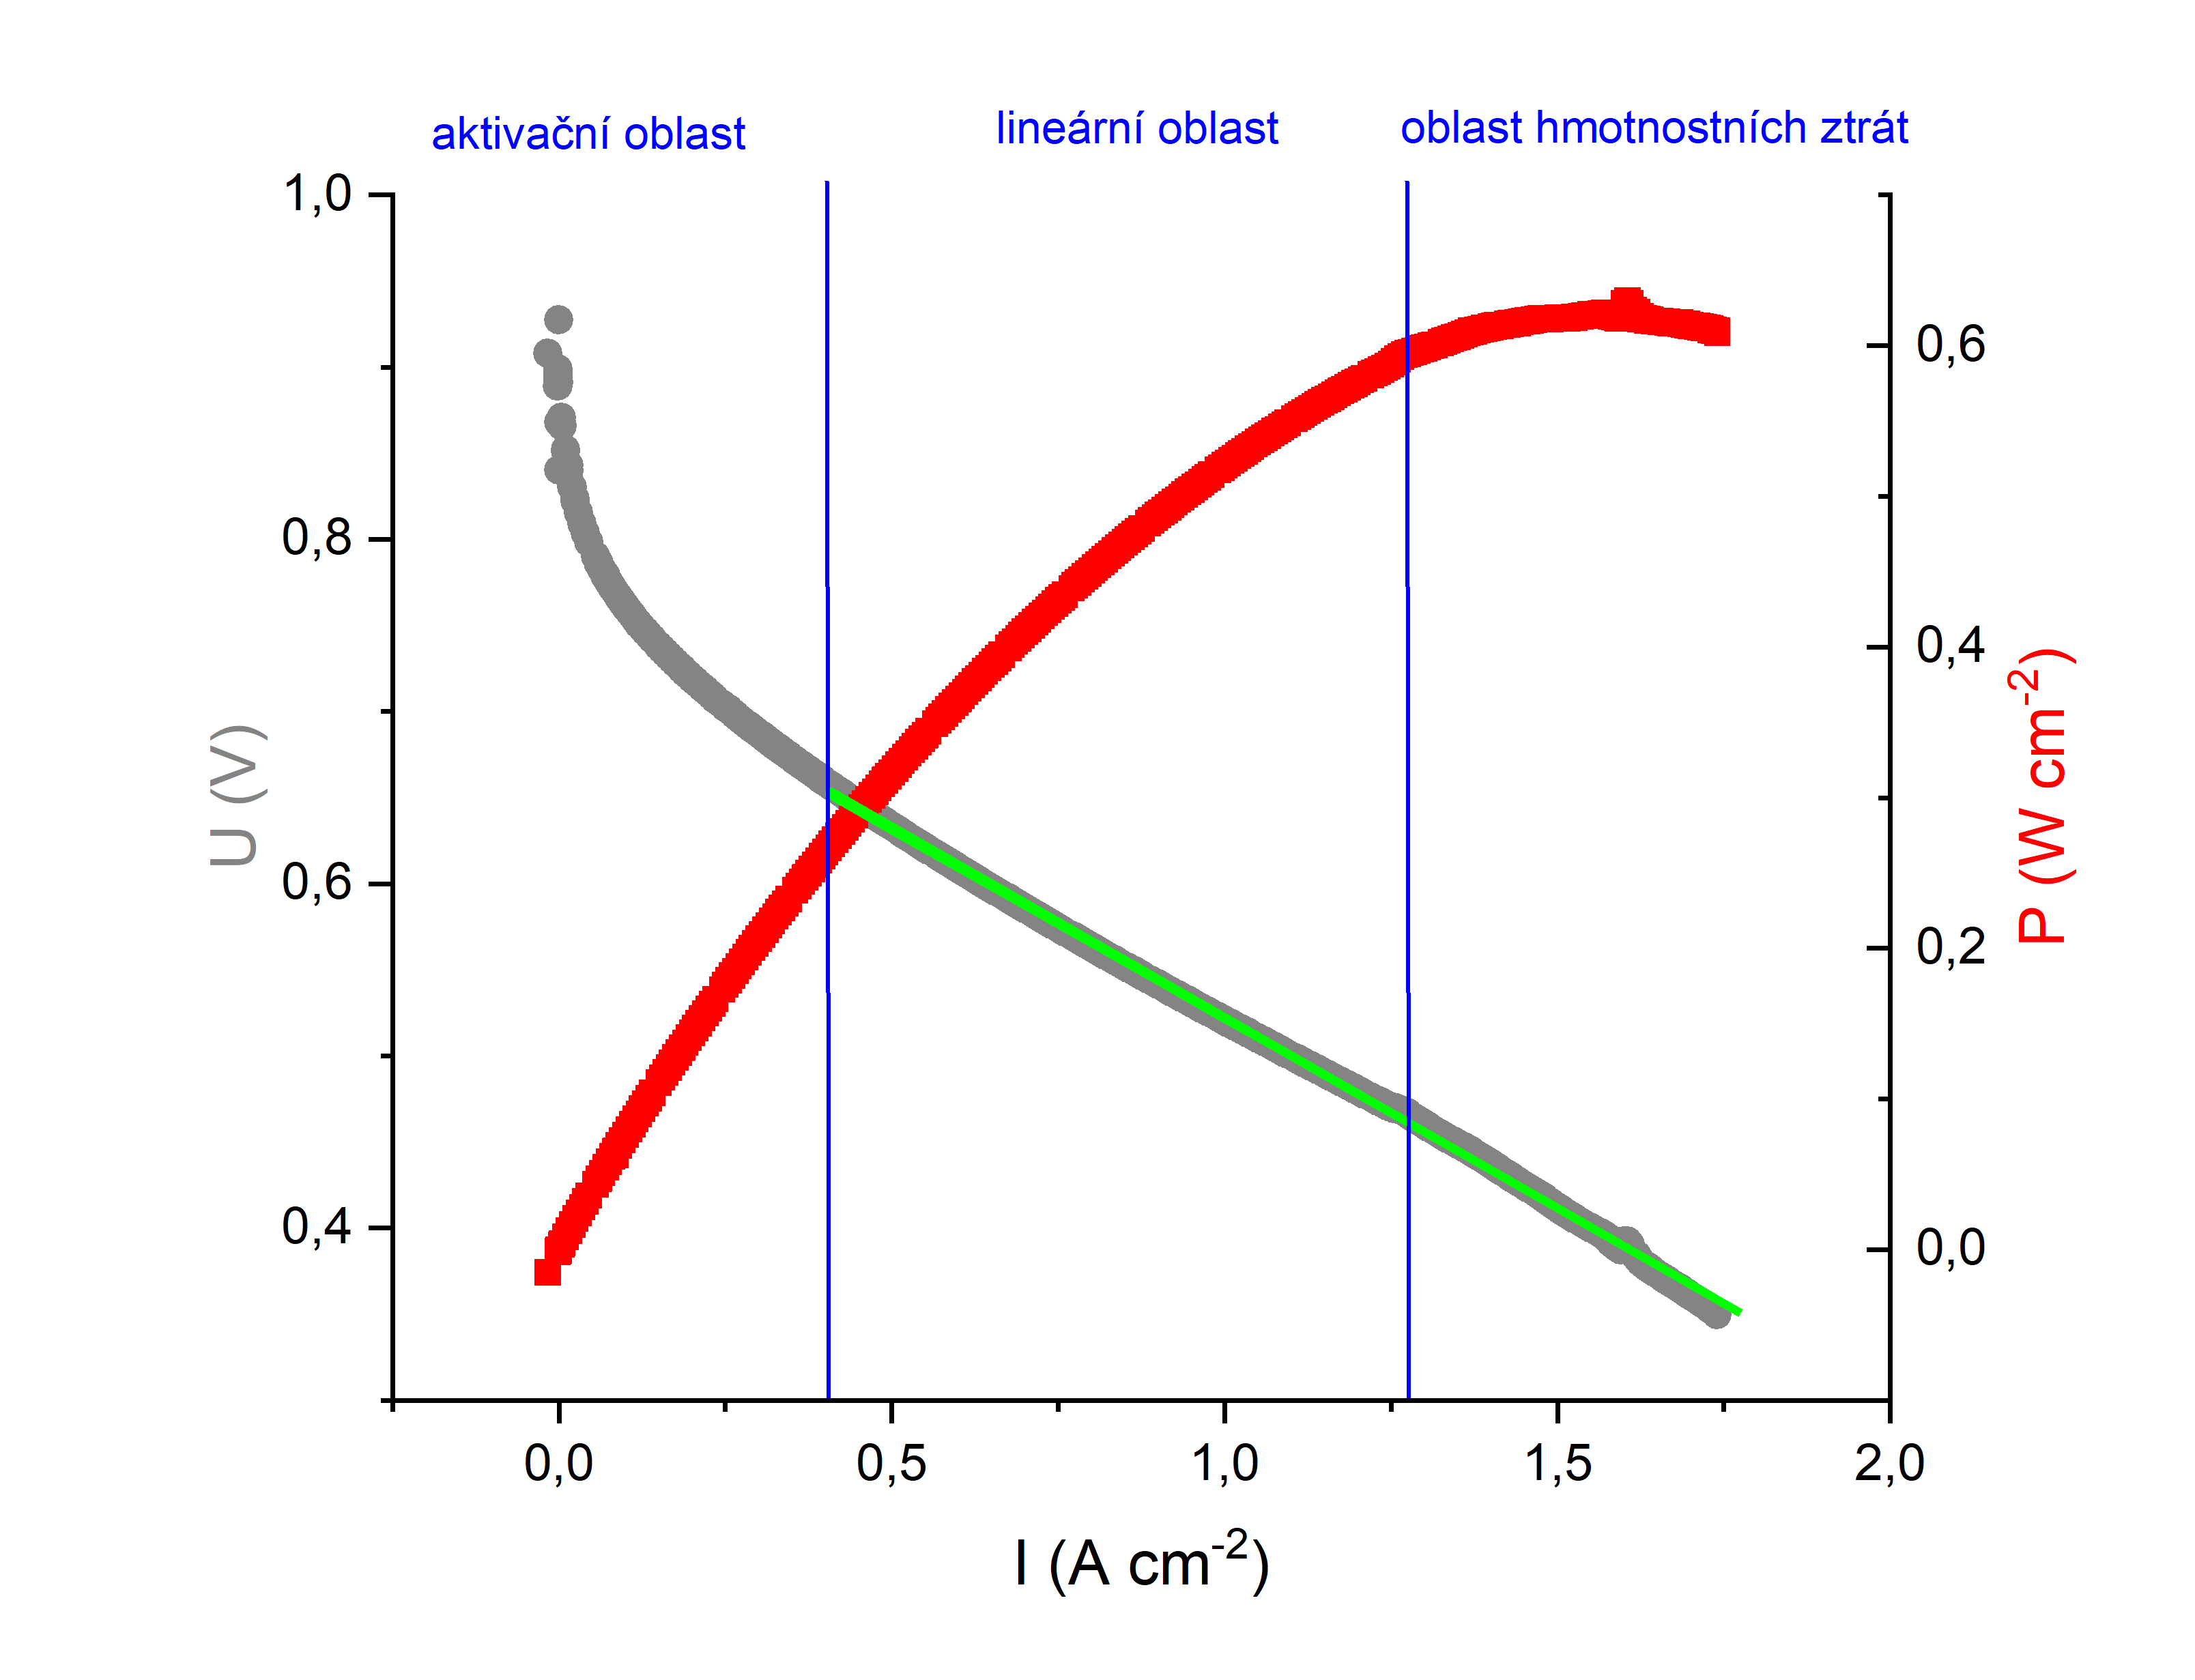
\includegraphics[width=1\linewidth]{H1 - vodíkový palivový článek/Polarizační křivka.png}
    \caption{Polarizační křivka a závislost výkonu}
    \label{fig:polar-krivk}
\end{figure}

    
% ----------------------------------------------------------------------
%  Diskuse výsledků
% ----------------------------------------------------------------------			
\section{Diskuse výsledků}

% ----------------------------------------------------------------------
%  Závěr
% ----------------------------------------------------------------------
\section{Závěr}
